\documentclass[compress,table,xcolor=table]{beamer}
\input{beamer_mirror.tex}
\begin{document}
% ------------------------------------------------------------------------------
\title{Reflection use-cases}
% - Intro/Recap ----------------------------------------------------------------
\section{Intro/Recap}
% ------------------------------------------------------------------------------
\frame{\titlepage}
\begin{frame}
  \frametitle{Contents}
  \begin{itemize}
    \item Metadata, metaobjects, reflections, \say{un-reflection}
    \item Parsing of application options 
    \begin{itemize}
      \smaller
      \item from command-line arguments,
      \item from configuration files
    \end{itemize}
    \item \ldots
  \end{itemize}
\end{frame}
% ------------------------------------------------------------------------------
\begin{frame}
  \frametitle{Metadata}
  \framesubtitle{describing program declarations}
  \larger
  \begin{itemize}
    \item type of a variable,
    \item data members of a \inlinecode{struct},
    \item constructors or member functions of a \inlinecode{class},
    \item base classes of a \inlinecode{class},
    \item return type of a function,
    \item parameters of a function,
    \item enumerators in an \inlinecode{enum} type,
    \item name of a namespace, type, function, data member, parameter, etc.
    \item address of a variable, data member or member function,
    \item specifier like \inlinecode{virtual}, \inlinecode{constexpr},
      \inlinecode{static}, etc.
    \item source location,
    \item \ldots
  \end{itemize}
\end{frame}
% ------------------------------------------------------------------------------
\begin{frame}[fragile]
  \frametitle{Metaobject}
  \begin{itemize}
    \item A {\em meta-level} representation of a {\em base-level} entity\footnote{
      namespace, type, class, function, constructor, destructor, variable,
        enumerator, expression, \ldots}
    \item On the {\em meta-level\footnote{unlike the base-level (namespaces,
      constructors, etc)}} all of the above are \say{reified}
    \item We say a metaobject \say{reflects} the {\em base-level} entity
    \item Provides access to {\em metadata} describing the reflected
      {\em base-level} entity
    \item A compile-time constant
    {\larger value} of a type satisfying the~following concept:
  \end{itemize}
  \begin{lstlisting}[language=c++2x]
template <typename X>
concept (*@\listinghl{metaobject}@*) = (*@{\em not-really-important-here}@*);
  \end{lstlisting}
\end{frame}
% ------------------------------------------------------------------------------
\begin{frame}[fragile]
  \frametitle{Reflection~~~~~~~~~~~~~~~~~~~~~~~\ldots and
  \say{un-reflection}\footnote{a.k.a. \say{"splicing"}}}
  \begin{columns}
    \begin{column}{.50\textwidth}
      \begin{itemize}
        \item The process of obtaining metadata or metaobjects which provide metadata
          indirectly
        \item Done through a~dedicated operator or~language expression
        \item For example
  \begin{lstlisting}[language=c++2x,basicstyle=\footnotesize\ttfamily]
auto (*@\listinghlt{meta_string}@*) =
  (*@\listinghl{mirror}@*)(std::string);
  \end{lstlisting}
      \end{itemize}
    \end{column}
    \begin{column}{.50\textwidth}
      \begin{itemize}
        \item Getting back to the base-level entity reflected by a metaobject
        \item \ldots through an operation on a metaobject reflecting that
          {\em base-level} entity
        \item \say{Splicing} can also mean emitting a snippet of code involving
          base-level entities, reflected by metaobjects
      \end{itemize}
    \end{column}
  \end{columns}
\end{frame}
% ------------------------------------------------------------------------------
\begin{frame}[fragile]
  \frametitle{Reflection API}
  \larger
  Set of compile-time\footnote{\inlinecode{consteval}, \inlinecode{constexpr}
    assumed, but omitted here to save space on slides}
   functions operating on {\em metaobjects}
  \smaller
  \begin{columns}
    \begin{column}{.50\textwidth}
      \begin{itemize}
        \item classification
          \begin{itemize}
            \smaller
            \item \inlinecode{reflects_type}, \inlinecode{reflects_callable},
              \ldots
          \end{itemize}
        \item primitive operations
          \begin{itemize}
            \smaller
            \item \inlinecode{get_name}, \inlinecode{get_scope},
            \item \inlinecode{get_type}, \inlinecode{get_aliased},
              \inlinecode{get_enumerators}, \inlinecode{is_constexpr},
              \inlinecode{is_scoped_enum},
              \inlinecode{is_pure_virtual}, \ldots
          \end{itemize}
        \item sequence operations
          \begin{itemize}
            \smaller
            \item \inlinecode{is_empty}, \inlinecode{get_size},
              \inlinecode{get_element}, \inlinecode{concat}, \ldots
          \end{itemize}
      \end{itemize}
    \end{column}
    \begin{column}{.50\textwidth}
      \begin{itemize}
        \item algorithms
          \begin{itemize}
            \smaller
            \item \inlinecode{for_each}, \inlinecode{fold},
              \inlinecode{join}, \inlinecode{transform},
              \inlinecode{filter}, \inlinecode{remove_if},
              \inlinecode{find_if}, \inlinecode{find_if_not},
              \inlinecode{find_ranking}, \ldots
          \end{itemize}
        \item comparators
          \begin{itemize}
            \smaller
            \item \inlinecode{reflects_same}, \ldots
          \end{itemize}
        \item syntax sugar, placeholder expressions
          \begin{itemize}
            \smaller
            \item \inlinecode{_1}, \inlinecode{_2},
              \inlinecode{get_type(_1)}, \inlinecode{reflects_same(_1, _2)},
              \ldots
          \end{itemize}
      \end{itemize}
    \end{column}
  \end{columns}
\end{frame}
% ------------------------------------------------------------------------------
\begin{frame}[fragile]
  \frametitle{\say{hello world of reflection!}}
  \begin{lstlisting}[language=c++2x,basicstyle=\normalsize\ttfamily]
enum class (*@\listinghlt{greeting}@*) {
  hello, world, of, reflection
};
  \end{lstlisting}
  \begin{lstlisting}[language=c++2x,basicstyle=\normalsize\ttfamily]
cout << (*@\listinghl{join\footnote{algorithm}}@*)(
          (*@\listinghl{get_enumerators\footnote{
            metaobject sequence getter}}@*)(mirror(*@\footnote{
            reflection operator}@*)((*@\listinghlt{greeting}@*))(*@\footnote{
            reflection in action -- returns a metaobject}@*)),
          to_string((*@\listinghl{get_name\footnote{
            metadata (name) getter}}@*)((*@\listinghlt{_1}@*)(*@\footnote{
            placeholder}@*)))(*@\footnote{
            placeholder expression}@*),
          string(" "))
       << "!\n";
  \end{lstlisting}
\end{frame}
% ------------------------------------------------------------------------------
% - Utilities ------------------------------------------------------------------
\section{Utilities}
% ------------------------------------------------------------------------------
\begin{frame}[fragile]
  \frametitle{\em Extractable}
  \framesubtitle{concepts}
  \larger
  \begin{itemize}
    \item Types which can optionally refer to or store a value
    \item Unifies usage of
    \begin{itemize}
      \item raw pointers, smart pointers,
      \item \inlinecode{optional}, \inlinecode{expected},
      \item \ldots
    \end{itemize}
    \item \ldots in some specific cases
  \end{itemize}
  \begin{lstlisting}[language=c++2x,basicstyle=\normalsize\ttfamily]
template <typename T>
concept extractable = requires(T v) {
	{ declval<(*@\listinghl{extracted_type_t}@*)<T>>() };
  { (*@\listinghl{has_value}@*)(v) } -> convertible_to<bool>;
  (*@\listinghl{extract}@*)(v);
};
  \end{lstlisting}
\end{frame}
% ------------------------------------------------------------------------------
\begin{frame}[fragile]
  \frametitle{\em Extractable}
  \framesubtitle{operations}
  \begin{itemize}
    \item \inlinecode{has_value_type} -- indicates if the extracted value has
      a~specific type
    \item \inlinecode{has_value} -- indicates if an extractable has a value
    \item \inlinecode{extract} -- provides access to a value in an extractable
  \end{itemize}
  \begin{lstlisting}[language=c++2x,basicstyle=\small\ttfamily]
template <typename V>
consteval auto has_value_type(
  const extractable auto& v)
  noexcept -> bool;
  \end{lstlisting}
  \vfill
  \begin{lstlisting}[language=c++2x,basicstyle=\normalsize\ttfamily]
auto has_value(
  extractable auto &) noexcept -> bool;
  \end{lstlisting}
  \begin{lstlisting}[language=c++2x,basicstyle=\footnotesize\ttfamily]
auto extract(extractable auto&) -> auto&;
auto extract(extractable auto&&) -> const auto&&;
auto extract(extractable const auto&) -> const auto&;
  \end{lstlisting}
\end{frame}
% ------------------------------------------------------------------------------
\begin{frame}[fragile]
  \frametitle{\em Extractable}
  \framesubtitle{the idiom}
  This is quite common\ldots
  \begin{lstlisting}[language=c++2x,basicstyle=\normalsize\ttfamily]
  auto (*@\listinghlt{get_opt_val}@*)(auto... params)
  -> (*@\listinghl{extractable}@*);
  \end{lstlisting}
  \vfill
  \begin{lstlisting}[language=c++2x,basicstyle=\normalsize\ttfamily]
  if(const auto opt{(*@\listinghlt{get_opt_val}@*)(args...)};
     (*@\listinghl{has_value}@*)(opt)) {

    do_something((*@\listinghl{extract}@*)(opt));
  } else {
    do_something_else();
  }
  \end{lstlisting}
\end{frame}
% ------------------------------------------------------------------------------
\begin{frame}[fragile]
  \frametitle{Conversion from string}
  \begin{lstlisting}[language=c++2x,basicstyle=\normalsize\ttfamily]
template <typename T>
auto from_string(
  const string_view src,
  type_identity<T> = {})
  -> (*@\listinghl{extractable}@*);
  \end{lstlisting}
  \vfill
  \begin{lstlisting}[language=c++2x,basicstyle=\normalsize\ttfamily]
template <typename T>
auto from_extractable_string(
  const (*@\listinghl{extractable}@*) auto src,
  type_identity<T> tid = {})
  -> (*@\listinghl{extractable}@*)
  requires((*@\listinghl{has_value_type}@*)<string_view>(src));
  \end{lstlisting}
\end{frame}
% ------------------------------------------------------------------------------
\begin{frame}[fragile]
  \frametitle{Command-line arguments}
  \begin{columns}
    \begin{column}{.57\textwidth}
      \begin{lstlisting}[language=c++2x,basicstyle=\scriptsize\ttfamily]
class program_arg {
public:
  auto next() -> program_arg;

  auto is_short_tag(
    string_view) -> bool;
  auto is_long_tag(
    string_view) -> bool;
  // ...
  operator string_view();
};
      \end{lstlisting}
      \vfill
      \begin{lstlisting}[language=c++2x,basicstyle=\scriptsize\ttfamily]
class program_args {
public:
  program_args(int, const char**);
  auto begin();
  auto end();
  auto command() -> string_view;
  // ...
  auto find(string_view)
    -> program_arg;
};
      \end{lstlisting}
    \end{column}
    \begin{column}{.44\textwidth}
      \small
      \begin{itemize}
        \item \inlinecode{program_arg} -- represents a single program argument.
        \begin{itemize}
          \smaller
          \item get previous and next argument,
          \item check for \verb@-o@ and \verb@--long-opt@ options,
          \item starts-with, ends-with,
          \item \ldots
        \end{itemize}
        \item \inlinecode{program_args} -- represents all program arguments
        \begin{itemize}
          \smaller
          \item iteration, search,
          \item command, first, last,
          \item \ldots
        \end{itemize}
      \end{itemize}
    \end{column}
  \end{columns}
\end{frame}
% - Parsing options ------------------------------------------------------------
\section{Args}
% ------------------------------------------------------------------------------
\begin{frame}[fragile]
  \frametitle{Parsing command-line arguments}
  \framesubtitle{into a structure}
  \small
  \begin{itemize}
    \item \inlinecode{options} -- application-specific data structure
      storing options
    \item \inlinecode{parse_args} -- generic function that parses and stores
      command-line argument values into a structure
    \begin{itemize}
      \item can be implemented using reflection
    \end{itemize}
  \end{itemize}
  \begin{lstlisting}[language=c++2x,basicstyle=\small\ttfamily]
struct options {
  string message{"Hello, world!"};
  chrono::milliseconds interval{500};
  int count{3};
};
  \end{lstlisting}
  \vfill
  \begin{lstlisting}[language=c++2x,basicstyle=\footnotesize\ttfamily]
template <typename T>
bool (*@\listinghl{parse_options}@*)(T& opts, const program_args&);
  \end{lstlisting}
\end{frame}
% ------------------------------------------------------------------------------
\begin{frame}[fragile]
  \frametitle{Parsing command-line arguments}
  \framesubtitle{usage}
  \begin{lstlisting}[language=c++2x,basicstyle=\footnotesize\ttfamily]
int main(int argc, const char** argv) {
    const (*@\listinghl{program_args}@*) args{argc, argv};
    (*@\listinghl{options}@*) (*@\listinghlt{opts}@*);

    if((*@\listinghl{parse_options}@*)((*@\listinghlt{opts}@*), args)) {
      const auto repeats{
        ranges::views::iota(1, opts.(*@\listinghlt{count}@*) + 1)};

      for(auto i : repeats) {
          cout << i << ": "
               << opts.(*@\listinghlt{message}@*) << endl;

          this_thread::sleep_for(opts.(*@\listinghlt{interval}@*));
      }
      return 0;
    } else {
      return 1;
    }
}  \end{lstlisting}
\end{frame}
% ------------------------------------------------------------------------------
\begin{frame}[fragile]
  \frametitle{Parsing arguments}
  \framesubtitle{how to implement {\em \larger generic} \inlinecode{parse_options}?}
  \begin{lstlisting}[language=c++2x,basicstyle=\scriptsize\ttfamily]
template <typename T>
bool parse_options(T& opts, const program_args& args) {
  bool parsed = true;

  for(const auto& arg : args) {
    (*@\listinghl{for_each}@*)((*@\listinghl{get_data_members}@*)((*@\listinghlt{mirror}@*)(T)), [&](auto mdm) {
      if(arg.is_long_tag((*@\listinghl{get_name}@*)(mdm))) {
        if(const auto opt{from_string(
          arg.next(), (*@\listinghl{get_reflected_type}@*)((*@\listinghl{get_type}@*)(mdm)))}
        ) {
           (*@\listinghl{get_reference}@*)(mdm, opts) = opt.value();
        } else {
            std::cerr << "invalid value '" << arg.next()
                      << "' for option " << arg
                      << "!" << std::endl;
            parsed = false;
        }
      }
    });
  }
  return parsed;
}
  \end{lstlisting}
\end{frame}
% - RPC ------------------------------------------------------------------------
\section{RPC}
% ------------------------------------------------------------------------------
\begin{frame}
  \frametitle{Remote procedure calls}
  \framesubtitle{class overview}
  \colorbox{gray}{
    \begin{minipage}{\dimexpr\textwidth\relax}
    \centering
    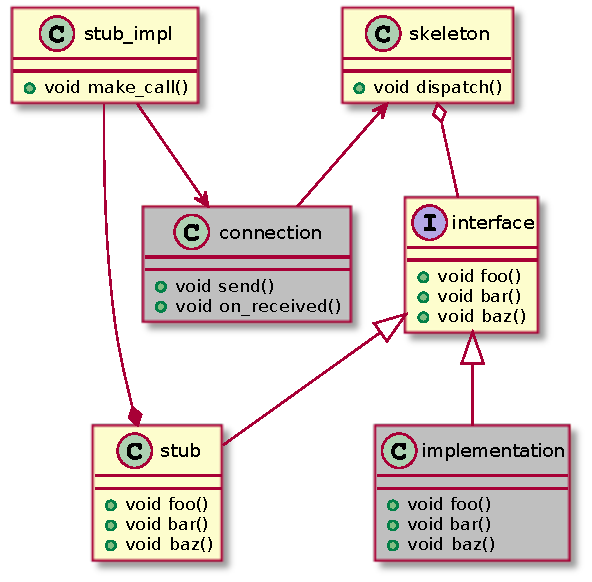
\includegraphics[
        width=0.65\textwidth,
        keepaspectratio
    ]{rpc_class.pdf}
    \end{minipage}
  }
\end{frame}
% ------------------------------------------------------------------------------
\begin{frame}
  \frametitle{Remote procedure calls}
  \framesubtitle{synchronous call sequence}
  \colorbox{lightgray}{
    \begin{minipage}{\dimexpr\textwidth\relax}
    \centering
    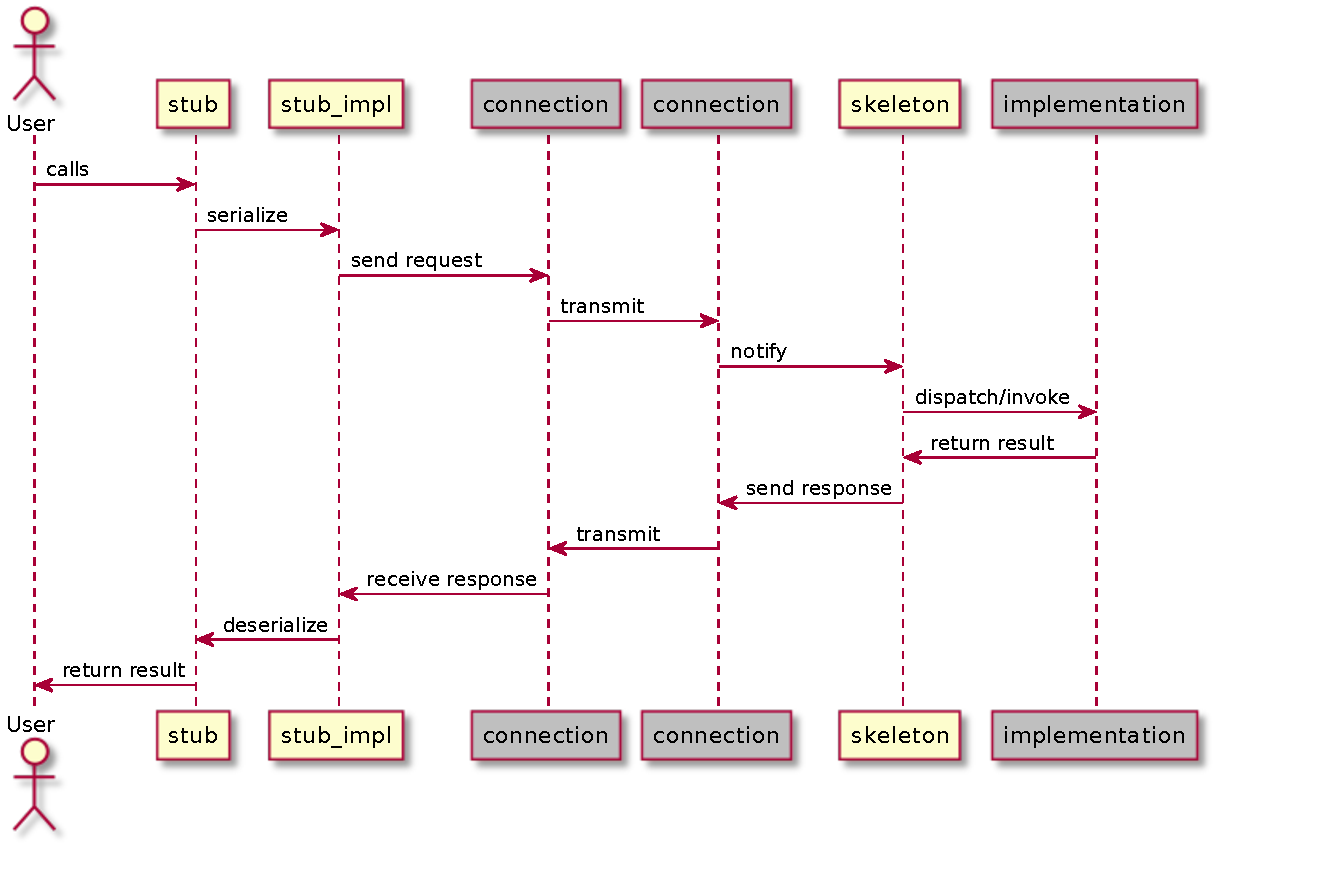
\includegraphics[
        width=0.9\textwidth,
        keepaspectratio
    ]{rpc_sequence.pdf}
    \end{minipage}
  }
\end{frame}
% ------------------------------------------------------------------------------
\begin{frame}[fragile]
  \frametitle{RPC stubs/skeletons}
  \framesubtitle{the interface}
  \begin{lstlisting}[language=c++2x,basicstyle=\small\ttfamily]
struct calculator {
    virtual float add(float, float) = 0;
    virtual float subtract(float, float) = 0;
    virtual float multiply(float, float) = 0;
    virtual float divide(float, float) = 0;
    virtual float negate(float) = 0;
    virtual float invert(float) = 0;
};
  \end{lstlisting}
\end{frame}
% ------------------------------------------------------------------------------
\begin{frame}[fragile]
  \frametitle{RPC stubs/skeletons}
  \framesubtitle{the stub}
  \begin{lstlisting}[language=c++2x,basicstyle=\footnotesize\ttfamily]
class calculator_stub : public calculator {
private:
    (*@\listinghl{rpc_stub_impl}@*) _impl;
public:
  float (*@\listinghlt{add}@*)(float l, float r) final {
    return _impl.(*@\listinghl{make_call}@*)(
      (*@\listinghl{mirror}@*)((calculator::(*@\listinghlt{add}@*)(l, r)))(*@\footnote{
        expression reflection}@*), l, r);
  }

  float (*@\listinghlt{subtract}@*)(float l, float r) final {
    return _impl.make_call(
      mirror((calculator::(*@\listinghlt{subtract}@*)(l, r))), l, r);
  }
  float multiply(float l, float r) final;
  float divide(float l, float r) final;
  float negate(float x) final;
  float invert(float x) final;
};
  \end{lstlisting}
\end{frame}
% ------------------------------------------------------------------------------
\begin{frame}[fragile]
  \frametitle{RPC stubs/skeletons}
  \framesubtitle{the generic stub implementation\footnote{pseudocode}}
  \begin{lstlisting}[language=c++2x,basicstyle=\footnotesize\ttfamily]
class rpc_stub_impl {
  template <typename T>
  auto _deserialize(packet&, (*@\listinghlt{type_identity}@*)<T>) -> T;
public:
  auto make_call(metaobject auto mo, auto&... args) {

    packet request;
    _serialize(request, mo, args...);
    packed response{_send_and_receive(request)};

    return _deserialize(
      response,
      (*@\listinghlt{get_reflected_type}@*)(
        (*@\listinghl{get_type}@*)(
          (*@\listinghl{get_callable}@*)(
            (*@\listinghl{get_subexpression}@*)(mo)))));
  }
};
  \end{lstlisting}
\end{frame}
% ------------------------------------------------------------------------------
% ------------------------------------------------------------------------------
\end{document}
